\documentclass[12pt,a4paper]{report}

% Essential packages
\usepackage[utf8]{inputenc}
\usepackage{placeins}
\usepackage[T1]{fontenc}
\usepackage{geometry}
\usepackage{setspace}
\usepackage{titlesec}
\usepackage{tocloft}
\usepackage{fancyhdr}
\usepackage{graphicx}
\usepackage{amsmath}
\usepackage{amsfonts}
\usepackage{newunicodechar}
\newunicodechar{⁻}{\textsuperscript{-}}
\usepackage{textcomp}
\usepackage{amssymb}
\usepackage{algorithm}
\usepackage{algorithmic}
\usepackage{listings}
\usepackage{xcolor}
\usepackage{booktabs}
\usepackage{array}
\usepackage{longtable}
\usepackage{multirow}
\usepackage{caption}
\usepackage{subcaption}
\usepackage{hyperref}
\usepackage{cleveref}
\usepackage[numbers]{natbib}
\usepackage{url}
\usepackage{enumitem}

% Page geometry
\geometry{
    left=3cm,
    right=2.5cm,
    top=2.5cm,
    bottom=2.5cm
}

% Line spacing
\onehalfspacing

% Header and footer
\pagestyle{fancy}
\fancyhf{}
\fancyhead[R]{\thepage}
\fancyhead[L]{\leftmark}
\renewcommand{\headrulewidth}{0.4pt}

% Chapter and section formatting
\titleformat{\chapter}[display]
{\normalfont\Large\bfseries\centering}{\chaptertitlename\ \thechapter}{20pt}{\Large}
\titlespacing*{\chapter}{0pt}{0pt}{20pt}

% Hyperref settings
\hypersetup{
    colorlinks=true,
    linkcolor=black,
    filecolor=magenta,      
    urlcolor=blue,
    citecolor=black,
    pdftitle={Master's Synopsis},
    pdfauthor={Your Name},
}


\newcommand{\university}{Indian Institute of Technology, Delhi}
\newcommand{\department}{Department of Applied Mechanics}
\newcommand{\degree}{Master of Science by Research}
\newcommand{\specialization}{Surrogate Modelling and Discrepancy Learning}
\newcommand{\thesistitle}{Multi-Fidelity Surrogate Modeling for Structural Response Prediction}
\newcommand{\authorname}{Abhijit Roy Choudhury}
\newcommand{\rollnumber}{2023AMY7542}
\newcommand{\supervisor}{Dr. Rajdip Nayek}
\newcommand{\cosupervisor}{Dr. Souvik Chakroborty} 
\newcommand{\submissiondate}{Aug, 2025}

\begin{document}

\begin{titlepage}
\centering
\vspace*{-1.5cm}
% Top line
\rule{\textwidth}{0.6pt} \\[0.3cm]
% Title 
{\LARGE \textbf{Multi-Fidelity Surrogate Modeling using Deep Learning for Structural Response Prediction}}
{\LARGE \textbf{and Damage Parameterization}}\\[0.25cm]

\rule{\textwidth}{0.6pt} \\[0.5cm]
% Report type
{\large \textsc{A SYNOPSIS REPORT}}\\[0.3cm]
{\normalsize Submitted in Partial Fulfillment of the Requirements\\
for the Degree of}\\[0.2cm]
{\large \textbf{Master of Science}}\\
{\large (by Research)}\\[0.08cm]
% Author details
\large by\\[0.2cm]
{\Large \textbf{Abhijit Roy Choudhury}}\\[0.08cm]
{\normalsize Roll No: \texttt{2023AMY7542}}\\[0.5cm]

% Supervisor details
{\normalsize Under the supervision of}\\[0.5cm]
{\large \textbf{Dr. Rajdip Nayek}}\\
{\large and}\\
{\large \textbf{Dr. Souvik Chakraborty}}\\[1 cm]
% Institute Seal (logo placeholder)
\includegraphics[width=3.8cm]{iit.png} \\[1 cm]
% Bottom info
{\large November 2025} \\[0.2cm]
{\large \textbf{Department of Applied Mechanics}}\\
{\large \textbf{Indian Institute of Technology Delhi}}
\end{titlepage}

% Abstract
\chapter*{Abstract}
Ensuring the safety of critical infrastructure hinges on our ability to detect damage in structures, a task traditionally hampered by immense operational costs. While computational simulation of wave propagation offers a powerful non-destructive testing approach, its practical application is often limited. High-fidelity simulations, such as 2D Finite Element Models (FEM), provide exceptional accuracy but demand significant computational resources, making them impractical for real-time analysis. Conversely, low-fidelity models, like a 1D zigzag theory approach, are computationally efficient but may lack the necessary precision for reliable damage characterization. This research addresses this trade-off by developing a sophisticated multi-fidelity surrogate model that synergistically combines the strengths of both simulation domains. The framework is initially trained on a large dataset of fast, low-fidelity 1D simulations to establish a foundational understanding of the physics. This knowledge is then refined and enhanced through fine-tuning with a smaller, high-quality dataset from expensive 2D FEM analyses. The resulting surrogate model, which integrates a deep learning autoencoder and an XGBoost regressor, can rapidly predict wave propagation responses for any given set of beam parameters. This capability is leveraged within an inverse problem solver, where an optimization algorithm iteratively adjusts notch parameters—specifically location, depth, and width—until the model's response matches the measured sensor data. By bridging the gap between computational accuracy and efficiency, this work presents a robust and accurate framework for real-time damage characterization, achieving high prediction accuracy and offering a practical solution for structural health monitoring.

\bigskip

\bigskip

\bigskip

\bigskip

\textbf{Keywords:} \textit{Structural Health Monitoring, Damage Detection, Multi-fidelity Modeling, Surrogate Model, Inverse Problem, Wave Propagation, Homogeneous Beams, Machine Learning, Finite Element Method, Deep Learning}

\newpage
\addcontentsline{toc}{chapter}{Abstract}


% Table of Contents
\tableofcontents
\newpage

% List of Figures
\listoffigures
\newpage

% List of Tables
\listoftables
\newpage

% List of Abbreviations (optional)
\chapter*{List of Abbreviations}
\addcontentsline{toc}{chapter}{List of Abbreviations}
\begin{tabular}{ll}

\end{tabular}
\newpage

% Main Content
\pagenumbering{arabic}
\setcounter{page}{1}

% Chapter 1: Introduction and Motivation
\chapter{Introduction and Motivation}
\label{chap:introduction}

\section{Background: Structural Health Monitoring (SHM) and Lamb Waves}
\label{Background}


Unprecedented infrastructure development driven by rapid societal growth has elevated the need of monitoring structural health from routine maintenance to a critical engineering priority. The gradual accumulation of damage, which often begins as minute defects and cracks, can pose a threat to the safety and longevity of critical infrastructure. Left undetected, these seemingly minor issues can propagate, leading to catastrophic structural failures. Traditional inspection methodologies, which rely on periodic and often visual assessments, are frequently inadequate for identifying these developing problems in their early stages. It is in this context that Structural Health Monitoring (SHM) has emerged as a revolutionary departure from conventional practices. Rather than relying on intermittent checks, SHM provides continuous, real-time assessment of a structure's condition through permanently installed sensor networks. The core principle involves constantly measuring how a structure responds to certain input(s), allowing for the detection of changes that indicate damage or deterioration. These systems collect vast amounts of data, extract meaningful features, and employ sophisticated pattern recognition algorithms to distinguish between healthy and damaged cases \citep{HUANG202248}. Modern SHM implementations have become essential in aerospace and maritime applications, particularly for aircraft structures and ship hulls where detecting minute damage at early stages is important \citep{Qing2019, silvacampillo2023health} The challenge in aircraft and ships is identifying cracks while they are still tiny, before they grow large enough to change how the structure vibrates or shift its natural frequencies. Early detection matters because waiting until cracks show up in vibration measurements means the damage has likely already reached a dangerous size, threatening the structural integrity of the aircraft during flight or the ship at sea\citep{Fan2021review}. The economic benefits of SHM are substantial, as early damage detection enables condition-based maintenance strategies that can significantly reduce lifecycle costs while simultaneously enhancing safety margins.


The effectiveness of SHM systems heavily depends on the chosen sensing technology, with ultrasonic guided waves, particularly Lamb waves, emerging as exceptionally powerful tools for damage detection in plate-like structures. Such plate-like geometries are ubiquitous in critical infrastructure, including aircraft fuselages, ship hulls, pressure vessels, and pipeline walls, where thin-walled construction offers strength while minimizing weight. Lamb waves are elastic waves that propagate along \textit{thin} plates, beams and shells, confined between the free surfaces of the structure. These guided waves carry both longitudinal and transverse displacement components, creating complex particle motion patterns that interact sensitively with structural discontinuities and damage. Lamb waves can propagate over long distances without significant energy loss, allowing large areas to be monitored with relatively few sensors  \citep{Philibert31122022, LU2024114666}.  

\begin{figure}[htbp]
    \centering
    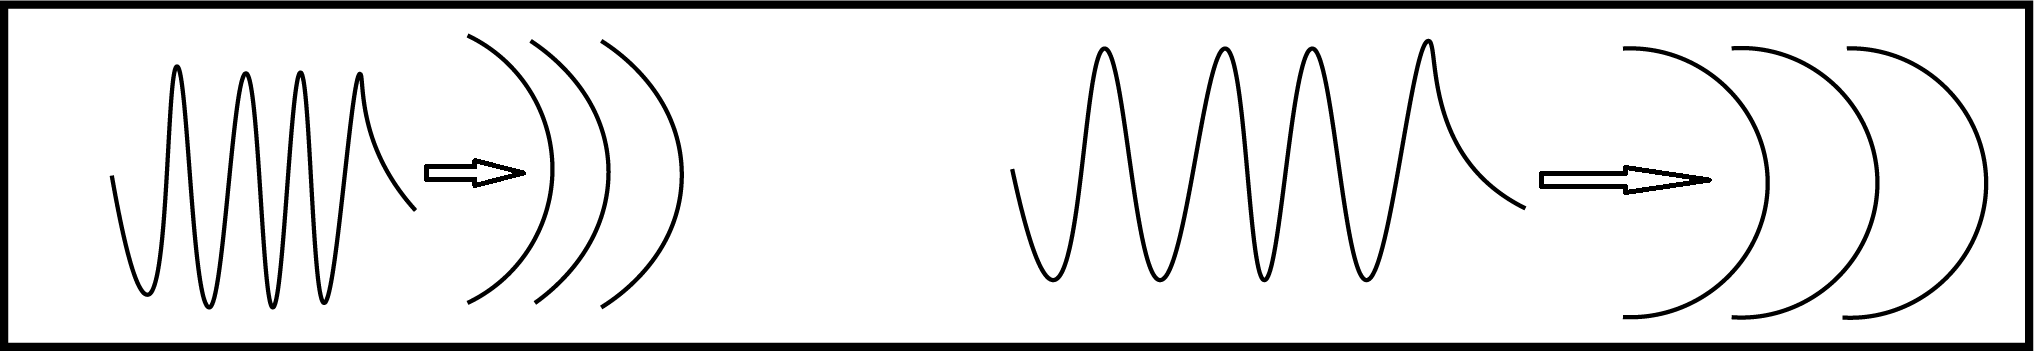
\includegraphics[width=0.8\textwidth]{Chapter1/lambwaves1.png}
    \caption{Lamb Waves Schematic \citep{rose2014ultrasonic}.}
    \label{fig:fig1}
\end{figure}

\begin{figure}[htbp]
    \centering
    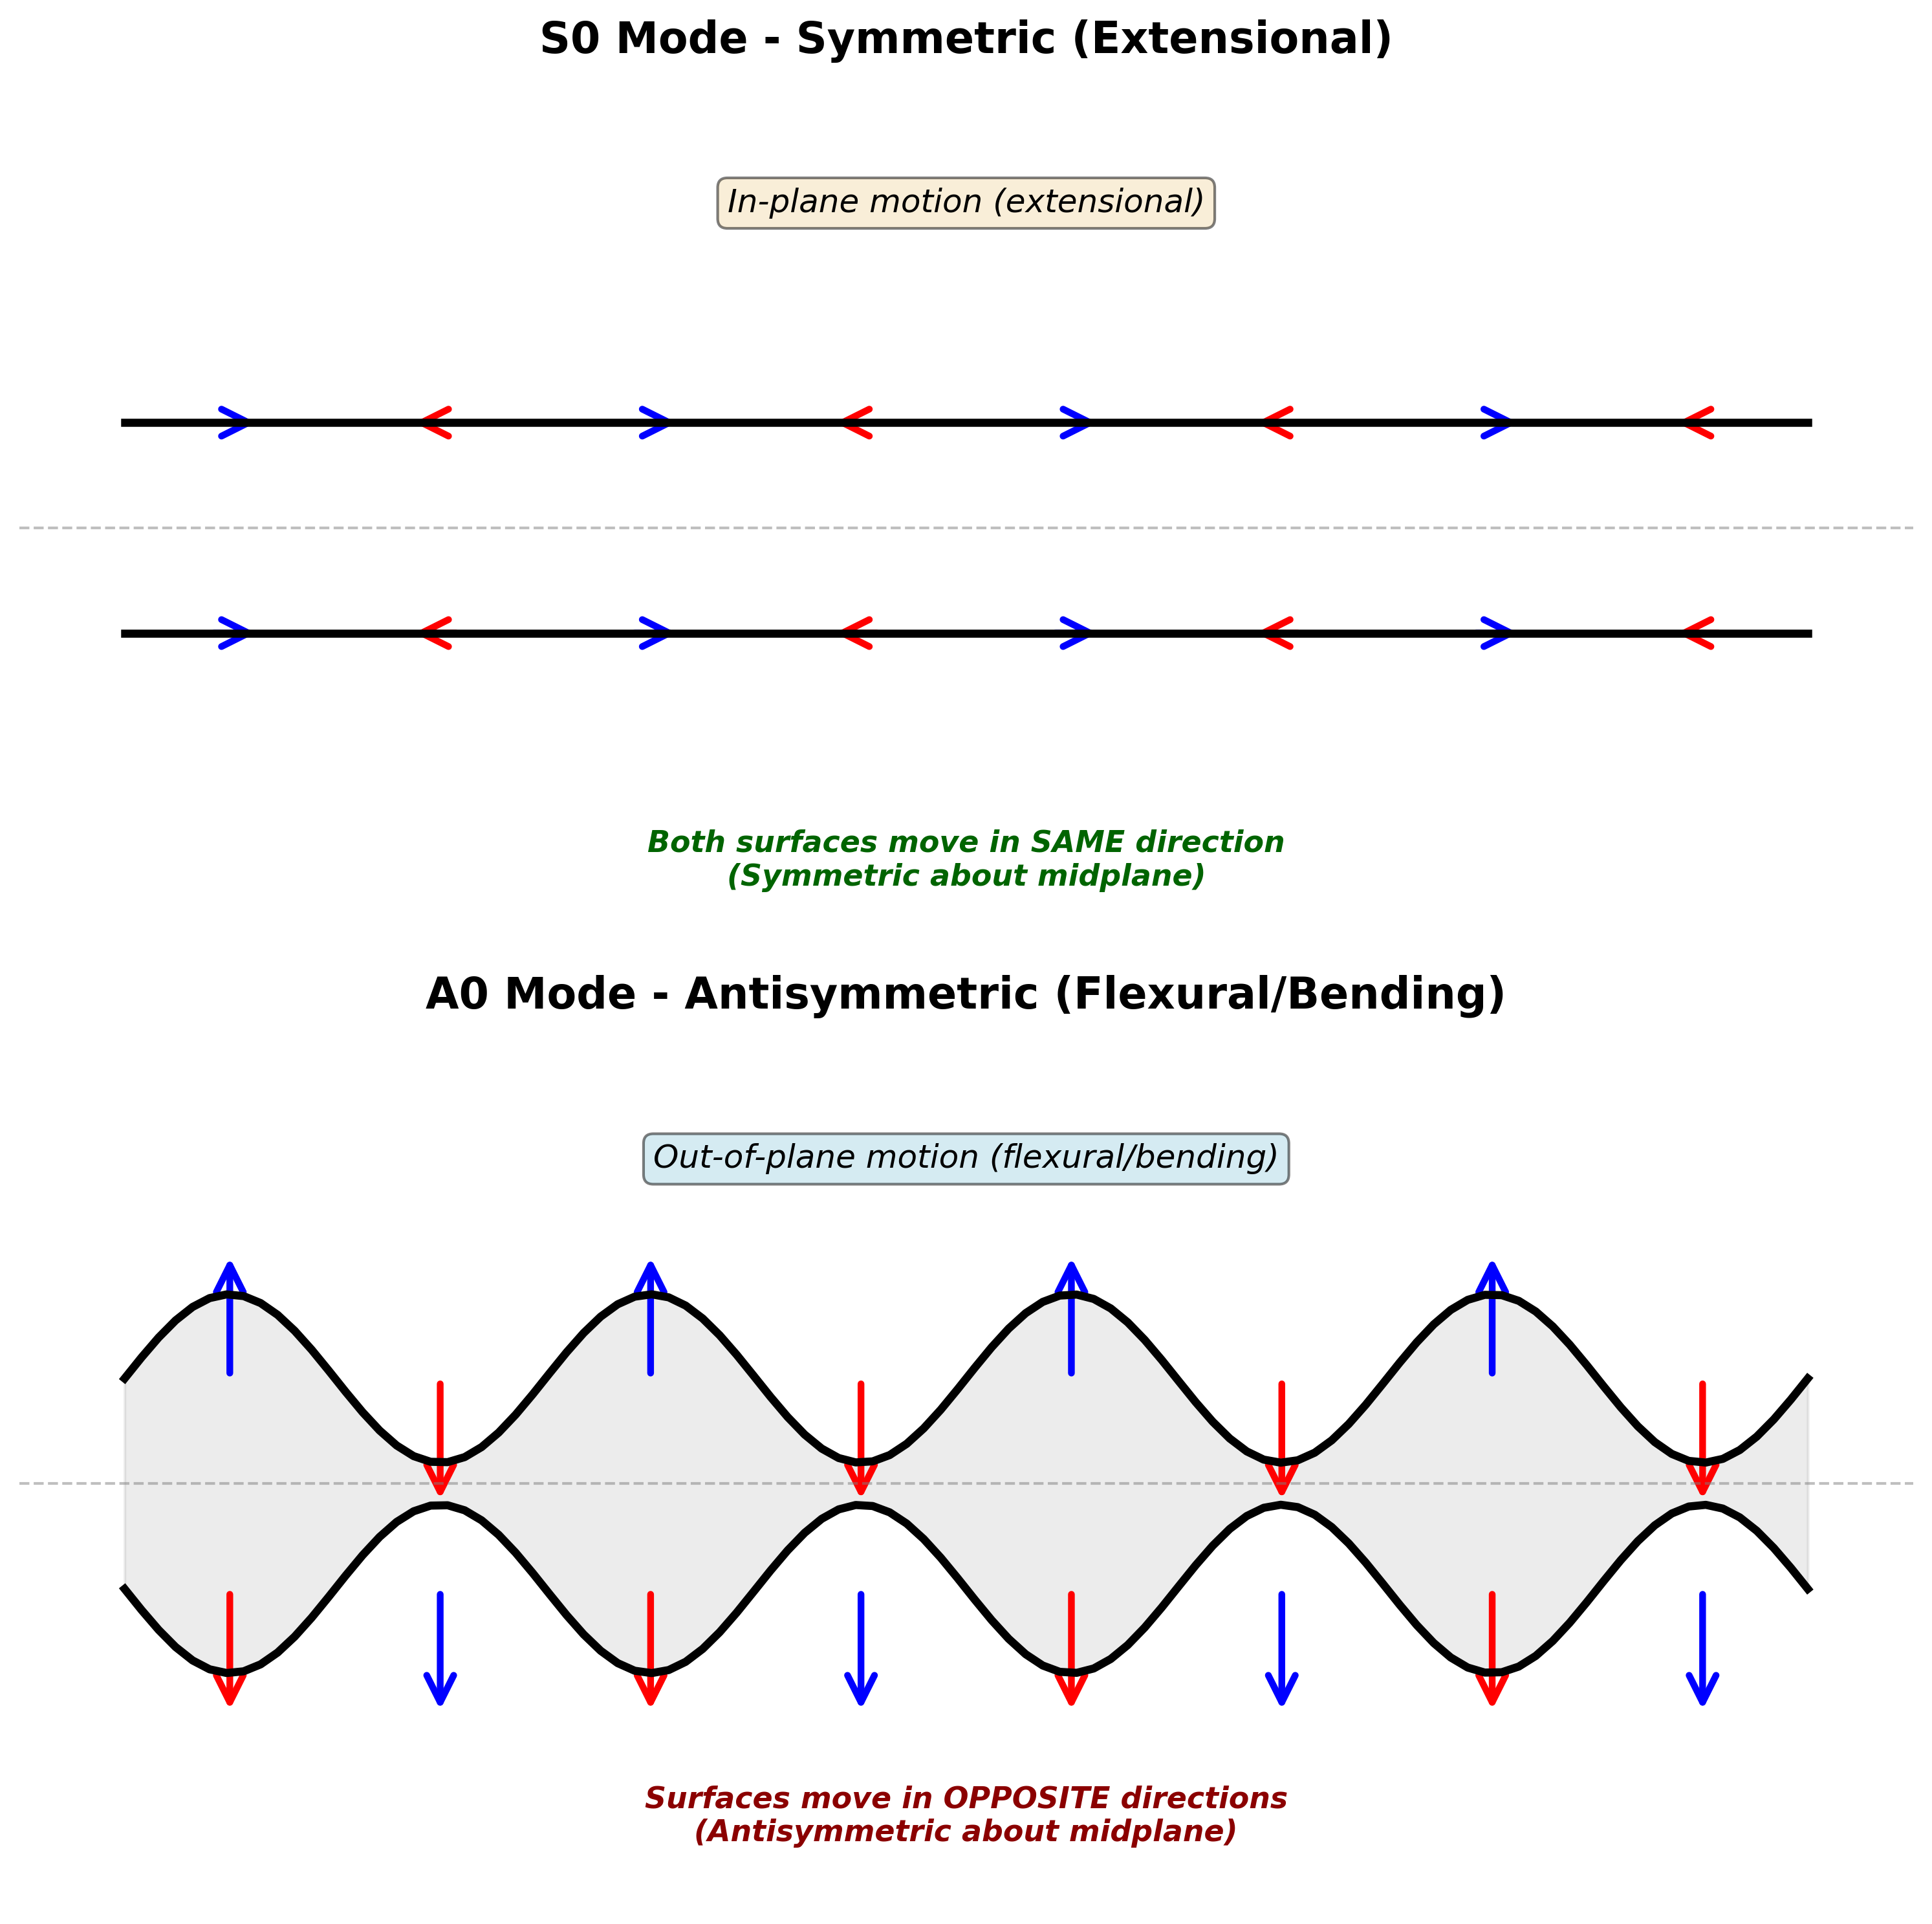
\includegraphics[width=0.8\textwidth]{Chapter1/A0_vs_S0_modes.png}
    \caption{Figure showing symmetric and anti-symmetric wavemodes \citep{rose2014ultrasonic}.}
    \label{fig:S0andA0}
\end{figure}

\FloatBarrier   % forces both to appear before the next section text

These waves demonstrate remarkable versatility in damage detection capabilities. The waves exist in two fundamental types: symmetric modes (S0, S1, S2, ...) and antisymmetric modes (A0, A1, A2, ...) as shown in Figure~\ref{fig:S0andA0}, with them being most important because they carry more energy than higher-order modes \citep{GIURGIUTIU2014293}. Symmetric modes exhibit particle motion that is symmetric about the plate's midplane, with predominantly in-plane displacement resembling extensional motion. Antisymmetric modes display motion that is antisymmetric about the midplane, characterized by out-of-plane displacement similar to flexural or bending motion. Damage sensing with Lamb waves is based on the observation of alteration in the signal waveform due to changes in the propagation  \citep{Muller2017}. 



However, practical implementation faces significant challenges. Analysis of signals acquired by ultrasonic transducers can be cumbersome because of the overlapping of multiple dispersive wave modes and complex wave propagation due to scattering. The computational demands for accurate modeling become particularly intensive when solving inverse problems to characterize damage from measured responses, necessitating advanced numerical techniques and significant computational resources.

\section{Challenges in Lamb-Wave Modeling for Damage Detection}
\label{challenges}

Developing computational models for Lamb wave propagation presents a fundamental trade-off that always has to be addressed. The pursuit of accuracy, particularly for high-frequency waves travelling over extended distances through structures mingled with subtle defects, must be balanced against computational efficiency and the demands of real-time analysis.

The core challenge lies in selecting the appropriate modeling approaches. Two-dimensional finite element models excel at capturing the physics of wave propagation with exceptional detail. These models account for complex wave interactions, multiple mode conversions, and the subtle effects of structural discontinuities that one-dimensional approaches fundamentally cannot represent \citep{Fan2024}. However, this computational fidelity demands substantial resources. High-frequency content requires fine spatial and temporal discretization, leading to simulation times that can extend from hours to days for a single analysis. Such computational requirements render 2D models impractical for the iterative processes inherent in damage detection applications.

One-dimensional models present an attractive alternative, operating orders of magnitude faster while providing reasonable approximations for certain wave propagation scenarios. Nevertheless, these simplified approaches sacrifice the important and complex physics that render Lamb waves particularly sensitive to structural changes. The resulting question becomes whether this sensitivity loss is acceptable when detecting potentially critical damage.

This computational dilemma intensifies when considering that damage detection constitutes an inverse problem by nature. Rather than executing a single simulation, the process requires hundreds or thousands of model evaluations as optimization algorithms search for damage parameters that best explain measured data \citep{YU2023107030}. Each iteration demands a forward model evaluation (in our case), causing computational costs to accumulate rapidly. Or work with the mildly accurate 1D model, which would often give incorrect estimation. These are called Low Fidelity Models (LFM). Engineers working with real structures often encounter this unavoidable constraint: employ high-fidelity 2D models (HFM) and await results over days, or accept the physical limitations of 1D LFM approximations with the risk of missing critical damage indicators.

Surrogate modeling strategies emerge as a response to these limitations. Surrogate models are computationally inexpensive approximations constructed by training mathematical functions on datasets generated from physics-based simulations. Low-fidelity surrogates utilize simplified mathematical representations or reduced-order models, while multi-fidelity approaches combine information from multiple model types with varying computational costs and accuracies. Unlike high-fidelity models that solve governing equations directly, these surrogates employ techniques such as polynomial regression, neural networks, or Gaussian process regression to approximate complex physical relationships. The objective involves preserving the essential physics captured by 2D models while achieving computational efficiency that approaches or even surpasses the speeds of 1D approximations.

\section{Limitations of Single Fidelity Simulations and their Surrogates}
\label{Limitations of surrogates}

Single-fidelity surrogate models face fundamental challenges when high-fidelity physics-based simulations become computationally prohibitive. Constructing accurate surrogates requires sufficiently large training datasets from expensive simulations, which becomes impractical for computationally intensive problems where individual runs extend to several hours \citep{Giselle_Fern_ndez_Godino_2023} \citep{Wang2020}. The problem worsens when dealing with multiple input parameters. As the parameters increase, the amount of training data needed grows exponentially to maintain accuracy \citep{Jakeman2020}. For example, structural health monitoring applications involving Lamb wave propagation demand thousands of model evaluations, making single-fidelity approaches computationally unaffordable \citep{https://doi.org/10.1002/eqe.4116}. Conversely, constructing surrogates purely from low-fidelity models, while computationally attractive, risks substantial inaccuracy or distortion of system response when simplified models fail to capture critical phenomena such as nonlinear wave interactions \citep{ZHANG2022101430}.

To enable practical and scalable Structural Health Monitoring (SHM) frameworks, there is a need for an integrated multi-fidelity modeling approach that:
\begin{enumerate}
    \item Utilizes simplified beam-theory-based low-fidelity (LF) models to efficiently generate wave-response data,
    \item Retains the predictive precision of high-fidelity (HF) models through selective fusion of high-fidelity information, and
    \item Employs machine-learning-based surrogate modeling for rapid forward and inverse predictions across a range of damage scenarios.
\end{enumerate}


To enable practical and scalable Structural Health Monitoring (SHM) frameworks, there is a need for an integrated multi-fidelity modeling approach that:
\begin{enumerate}
    \item Utilizes simplified beam-theory-based low-fidelity (LF) models to efficiently generate wave-response data,
    \item Retains the predictive precision of high-fidelity (HF) models through selective fusion of high-fidelity information, and
    \item Employs machine-learning-based surrogate modeling for rapid forward and inverse predictions across a range of damage scenarios.
\end{enumerate}

The central problem addressed in this thesis is therefore:

\medskip

\textbf{"To develop a computationally efficient, physics-consistent multi-fidelity surrogate modeling framework for accurate forward prediction and inverse identification of Lamb-wave responses in thin plate-like structures with surface-level damages."}

\section{Motivation and Research Gap}
\label{Research Gap}




\section{Research Objectives}

This research aims to develop and validate a bi-fidelity surrogate modeling framework for structural response prediction in notched beam configurations and to apply this framework for efficient notch parameter identification in Lamb-wave-based SHM applications.

\bigskip

\noindent\textbf{Research Objectives}

\begin{itemize}
    \item \textbf{Develop Bi-Fidelity Computational Models}
    \begin{itemize}
        \item Extend Refined Zigzag Theory to model notched homogeneous aluminum beams with FEM discretization
        \item Generate comprehensive parametric datasets for surrogate model training
        \item Establish high-fidelity 2D FE reference solutions with matched sensor/actuator configurations
    \end{itemize}
    
    \item \textbf{Create Machine Learning Surrogate Architectures}
    \begin{itemize}
        \item Develop low-fidelity surrogate model using autoencoders and XGBoost for rapid response prediction
        \item Implement a bi-fidelity surrogate model using transfer learning on the existing Low Fidelity Surrogate Model to capture discrepancies between modeling fidelities
    \end{itemize}
    
    \item \textbf{Develop Inverse Problem Solver for Structural Health Monitoring}
    \begin{itemize}
        \item Create inverse solver to estimate notch parameters from ultrasonic wave responses
        \item Implement differential evolution optimization to minimize discrepancies between predicted and measured responses and use the Multi Fidelity Surrogate Model as the Forward Problem to help estimate the parameters
        \item Validate performance through systematic testing on high-fidelity response data
    \end{itemize}
\end{itemize}

\section{Organization of the Thesis}


This thesis is structured into seven chapters. Chapter 2 explains the physics of Lamb waves and how they propagate through structures. It covers the basic wave modes, dispersion behavior, and how waves scatter when they encounter damage. The chapter also discusses why simulating these waves is computationally challenging.

Chapter 3 describes how the simulation data is generated using elastic beam theory. The numerical setup is detailed here, including mesh design, boundary conditions, and how notches are modeled. This chapter shows the difference between low-fidelity and high-fidelity simulation approaches and goes in depth about zigzag theory and its implementation in homogeneous beams.

The multi-fidelity modeling framework is presented in Chapter 4. It explains why combining different fidelity levels makes sense for structural health monitoring and reviews existing strategies like co-Kriging. The chapter then introduces the proposed framework and details how data from different sources is fused together. Training procedures and validation metrics are also covered.

Chapter 5 focuses on the machine learning methods used in this work. The autoencoder architecture is explained first, showing how it compresses wave response data into a compact representation. XGBoost is then introduced to model the relationship between damage parameters and these compressed features. The chapter demonstrates how these two components work together to form a complete prediction engine.

The practical application is demonstrated in Chapter 6 through a detailed case study. Different notch configurations are tested, and results from multi-fidelity and single-fidelity approaches are compared. The chapter evaluates both forward prediction accuracy and inverse problem notch parameters estimation. Physical interpretation of the results is emphasized throughout.

Chapter 7 concludes the thesis by summarizing key contributions and findings. Limitations of the current approach are discussed honestly, including assumptions about physics coverage and data requirements. Future research directions are suggested, such as experimental validation and integration with physics-informed neural networks.

\chapter{Fundamentals of Lamb Waves and its Role in SHM}

\section{Basics of Guided Ultrasonic Waves}

When mechanical disturbances propagate through infinite three-dimensional media, they travel as bulk waves-longitudinal waves that compress and extend the material, or shear waves that distort it transversally. However, when wave propagation occurs in structures with at least one dimension comparable to the wavelength, such as plates, shells, or beams, the wave behavior changes fundamentally. The boundaries of the structure constrain the wave motion, giving rise to \textit{guided ultrasonic waves}. These waves are ``guided'' in the sense that they propagate along the structure while being confined by its geometry, repeatedly reflecting between the surfaces and creating characteristic wave patterns.

The significance of guided waves in structural health monitoring (SHM) is substantial. Unlike bulk waves that propagate in all directions and dissipate rapidly, guided waves can travel long distances along a structure with relatively low  \citep{Yang2025Dataset}. This property enables a single transducer pair to interrogate large structural areas, making damage detection practical and cost-effective. In a typical SHM setup, an actuator generates a pulse that travels as a guided wave through the structure. Any discontinuity: a crack, delamination, or notch, causes partial reflection, mode conversion, and scattering of the incident wave. By analyzing the received signal at sensor locations, information about the damage can be extracted.

The mathematical description of guided waves begins with the equations of motion in an elastic medium. For a homogeneous, isotropic material, the displacement field $\mathbf{u}$ must satisfy the Navier-Cauchy equation:

\begin{equation}
\rho \frac{\partial^2 \mathbf{u}}{\partial t^2} = (\lambda + \mu) \nabla (\nabla \cdot \mathbf{u}) + \mu \nabla^2 \mathbf{u}
\end{equation}

where $\rho$ is the material density, and $\lambda$ and $\mu$ are the Lamé constants related to Young's modulus $E$ and Poisson's ratio $\nu$ through:

\begin{equation}
\lambda = \frac{E\nu}{(1+\nu)(1-2\nu)}, \quad \mu = \frac{E}{2(1+\nu)}
\end{equation}

For a structure with finite thickness, such as a plate of thickness $h$, traction-free boundary conditions must be imposed at the top and bottom surfaces. These conditions, combined with the equations of motion, lead to a characteristic equation that admits discrete solutions. Each solution represents a distinct wave mode with its own displacement profile through the thickness and its own relationship between frequency and wave speed, a relationship known as \textit{dispersion} \citep{rose2014ultrasonic}.

\begin{figure}[h!]
\centering
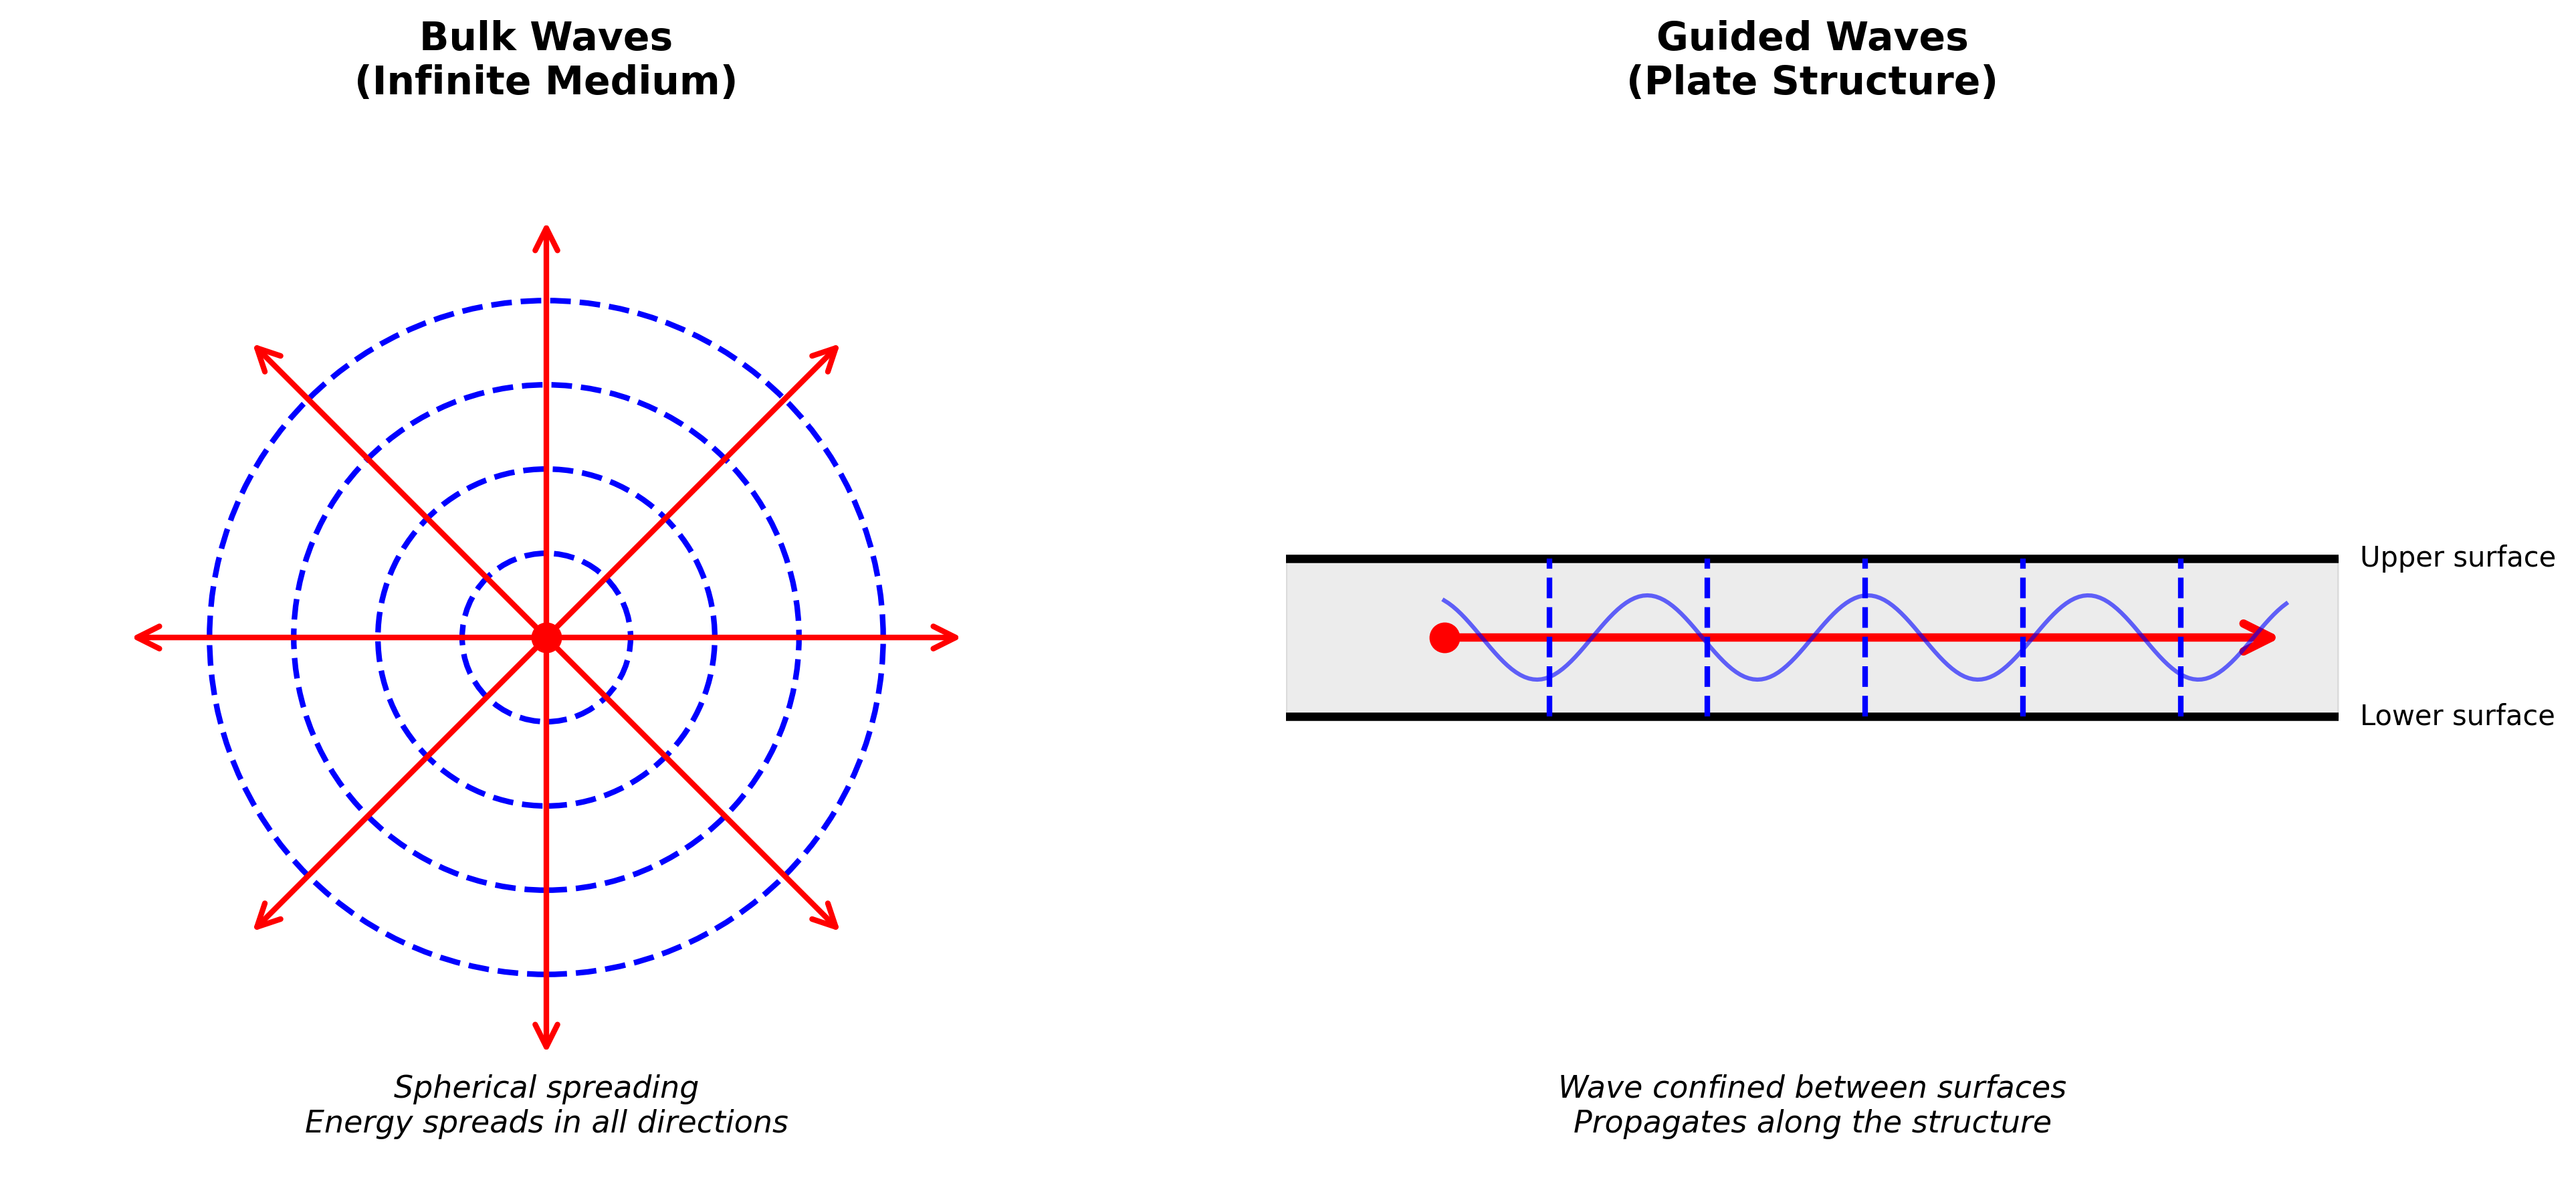
\includegraphics[width=1.0\textwidth]{Chapter2image/bulk_vs_guided_waves.png}
\caption{Schematic comparison of bulk waves vs guided waves}
\end{figure}

The energy carried by guided waves remains concentrated near the structure's surface, making them sensitive to surface-breaking defects and near-surface damage. Furthermore, because multiple modes can coexist at a given frequency, each with different velocity and displacement characteristics, careful selection of excitation frequency and mode allows tailoring the inspection to specific damage types and locations. This multimodal nature, while sometimes complicating signal interpretation, provides rich information about the structural condition when properly analyzed.

\section{Lamb Wave Modes (S\textsubscript{0} and A\textsubscript{0}'s Dispersion Behavior)}

Lamb waves, named after Horace Lamb who first derived their mathematical description in 1917, are a specific class of guided ultrasonic waves that propagate in thin plates or plate-like structures. Unlike surface waves such as Rayleigh waves that decay exponentially with depth, Lamb waves involve the entire thickness of the plate. They exist because the stress-free boundary conditions at both surfaces create standing wave patterns through the thickness, while the wave propagates freely along the plate.

The fundamental characteristic that distinguishes different Lamb wave modes is the symmetry of their displacement field with respect to the plate's midplane. Symmetric modes, denoted by $S$ with a numerical subscript ($S_0, S_1, S_2, \ldots$), exhibit displacement profiles that are symmetric about the midplane. In the fundamental symmetric mode $S_0$, particles on the top and bottom surfaces move in phase with each other. The through-thickness displacement pattern resembles extensional motion at low frequencies, with particles moving predominantly parallel to the propagation direction. Antisymmetric modes, denoted by $A$ with subscripts ($A_0, A_1, A_2, \ldots$), have displacement profiles that are antisymmetric about the midplane. The fundamental antisymmetric mode $A_0$ features out-of-phase motion between top and bottom surfaces, producing a flexural or bending-like deformation, especially at low frequencies.

The mathematical treatment begins with assuming harmonic wave solutions of the form:

\begin{equation}
\mathbf{u}(x, z, t) = \mathbf{U}(z)e^{i(kx - \omega t)}
\end{equation}

where $x$ is the propagation direction, $z$ is the through-thickness coordinate, $k$ is the wavenumber, and $\omega$ is the angular frequency. Substituting this into the governing equations and applying traction-free boundary conditions at $z = \pm h/2$ yields the Rayleigh-Lamb frequency equations. For symmetric modes:

\begin{equation}
\frac{\tan(\beta h/2)}{\tan(\alpha h/2)} = -\frac{4k^2 \alpha \beta}{(k^2 - \beta^2)^2}
\end{equation}

For antisymmetric modes:

\begin{equation}
\frac{\tan(\beta h/2)}{\tan(\alpha h/2)} = -\frac{(k^2 - \beta^2)^2}{4k^2 \alpha \beta}
\end{equation}

where $\alpha$ and $\beta$ are related to the wavenumber and material properties through:

\begin{equation}
\alpha^2 = \frac{\omega^2}{c_L^2} - k^2, \quad \beta^2 = \frac{\omega^2}{c_T^2} - k^2
\end{equation}

with $c_L = \sqrt{(\lambda + 2\mu)/\rho}$ being the longitudinal wave speed and $c_T = \sqrt{\mu/\rho}$ the shear wave speed \citep{SU2016353}.

These transcendental equations have no closed-form solutions and must be solved numerically for each frequency. Each solution corresponds to a mode with a specific wavenumber $k$, from which the phase velocity $c_p = \omega/k$ and group velocity $c_g = d\omega/dk$ can be determined. The resulting dispersion curves—plots of phase velocity or group velocity versus frequency—are fundamental to understanding Lamb wave behavior.


The dispersion behavior has profound implications for SHM applications. At low frequency-thickness products (typically $fd < 1$~MHz$\cdot$mm, where $f$ is frequency and $d$ is thickness), only the fundamental modes $S_0$ and $A_0$ propagate. The $S_0$ mode approaches the plate wave velocity at very low frequencies, exhibiting minimal dispersion, while the $A_0$ mode is highly dispersive, with its velocity approaching zero as frequency decreases. This means that an $A_0$ wavepacket will spread out significantly as it propagates, with higher frequency components traveling faster than lower frequencies.

The choice between $S_0$ and $A_0$ modes for damage detection involves tradeoffs. The $S_0$ mode's lower dispersion and higher velocity enable cleaner signals and faster inspection, making it favorable for large-area scanning. However, the $A_0$ mode's flexural nature makes it more sensitive to surface-breaking defects, delaminations, and thickness variations. In practice, excitation typically generates both modes simultaneously, and the resulting signal contains contributions from each mode arriving at different times due to their different group velocities. This multimodal nature can be exploited—by analyzing arrival times and amplitude changes of individual modes, more comprehensive damage characterization becomes possible than with single-mode analysis alone.

The computational challenge in predicting Lamb wave interactions with damage stems directly from this dispersion behavior. Time-domain finite element simulations must resolve multiple wavelengths with sufficient spatial discretization while tracking wave evolution over distances many times the plate thickness. The frequency-dependent velocities mean that narrow-band excitation produces relatively simple waveforms, while broadband pulses—often preferred for time-domain resolution—create complex, dispersive signals that require sophisticated post-processing. This computational burden motivates the development of surrogate models and multi-fidelity approaches, where expensive high-fidelity simulations are complemented by faster, approximate models to enable rapid damage detection and characterization.

\section{Wave Propagation and Scattering Due to Defects}

The utility of Lamb waves for structural health monitoring fundamentally relies on their interaction with structural discontinuities. When a propagating wave encounters damage—whether a crack, notch, delamination, or corrosion—the local change in geometry and material properties disrupts the wavefield. This disruption manifests as a combination of reflection, transmission, mode conversion, and scattering, each carrying information about the defect's characteristics \citep{rose2014ultrasonic,ahn2021lamb}. Understanding these interaction mechanisms is essential for interpreting measured signals and extracting damage parameters.

Consider a Lamb wave propagating along a structure and encountering a notch or through-thickness defect. The incident wave can be decomposed into symmetric and antisymmetric components, each with its own wavenumber and displacement profile. At the defect location, the stress-free boundary condition within the damage region cannot be satisfied by the incident wave alone. The wavefield must adjust to accommodate this new boundary, generating reflected and transmitted waves that travel away from the defect. The principle of superposition requires that the total displacement field—incident plus scattered waves—satisfies both the governing equations throughout the domain and the boundary conditions at all surfaces, including those created by the damage \citep{ahn2021lamb}.

The scattering process is inherently multimodal. Even if a pure $S_0$ mode impinges on a defect, the scattered field generally contains both $S_0$ and $A_0$ components, along with higher-order modes if the excitation frequency permits their propagation. This phenomenon, known as \textit{mode conversion}, occurs because the defect breaks the symmetry that would otherwise preserve modal purity \citep{ahn2021lamb}. A symmetric defect placed exactly at the plate midplane produces less mode conversion than an asymmetric defect or one located off-center, but some conversion typically occurs due to the complex three-dimensional stress redistribution around the damage \citep{cawley2018practical}.

The amplitude of reflected and transmitted waves depends on the defect's size relative to the wavelength. For damage dimensions much smaller than the wavelength, the defect acts as a point scatterer, with energy radiating in multiple directions but relatively weak reflection in the backward direction. As the defect size approaches or exceeds the wavelength, specular reflection becomes significant, and the scattered field develops directional characteristics \citep{rose2014ultrasonic}. This frequency-dependent interaction means that damage of a given size will interact more strongly with higher-frequency components of a broadband pulse, while lower frequencies may pass with minimal disturbance.

Quantitatively, the scattered wavefield can be expressed through the concept of \textit{scattering coefficients} \citep{ahn2021lamb}. For a defect at position $x_d$, the total displacement field can be written as:

\begin{equation}
u_{\text{total}}(x,z,t) = u_{\text{incident}}(x,z,t) + 
\sum_{m} R_m \, u_m^{\text{reflected}}(x,z,t) + 
\sum_{n} T_n \, u_n^{\text{transmitted}}(x,z,t)
\end{equation}

where the summations run over all propagating modes, and $R_m$ and $T_n$ are the reflection and transmission coefficients for modes $m$ and $n$, respectively. These coefficients are complex-valued, encoding both amplitude and phase changes. For a given incident mode and defect geometry, these coefficients can be determined through analytical methods for simple geometries or, more commonly, through numerical simulation for realistic damage scenarios \citep{ahn2021lamb,rose2014ultrasonic}.

The spatial distribution of the scattered field exhibits characteristic patterns. Directly behind the defect (in the forward direction), a shadow zone may form where the transmitted wave amplitude is reduced \citep{Im}. This amplitude reduction provides a direct measure of damage severity when sensors are positioned on opposite sides of the defect \citep{na2021review}. In the backward direction, the reflected wave interferes with the incident wave, creating standing wave patterns near the defect that contain information about the defect location through the phase relationship between incident and reflected components \citep{rose2014ultrasonic}.

\begin{figure}[h]
\centering
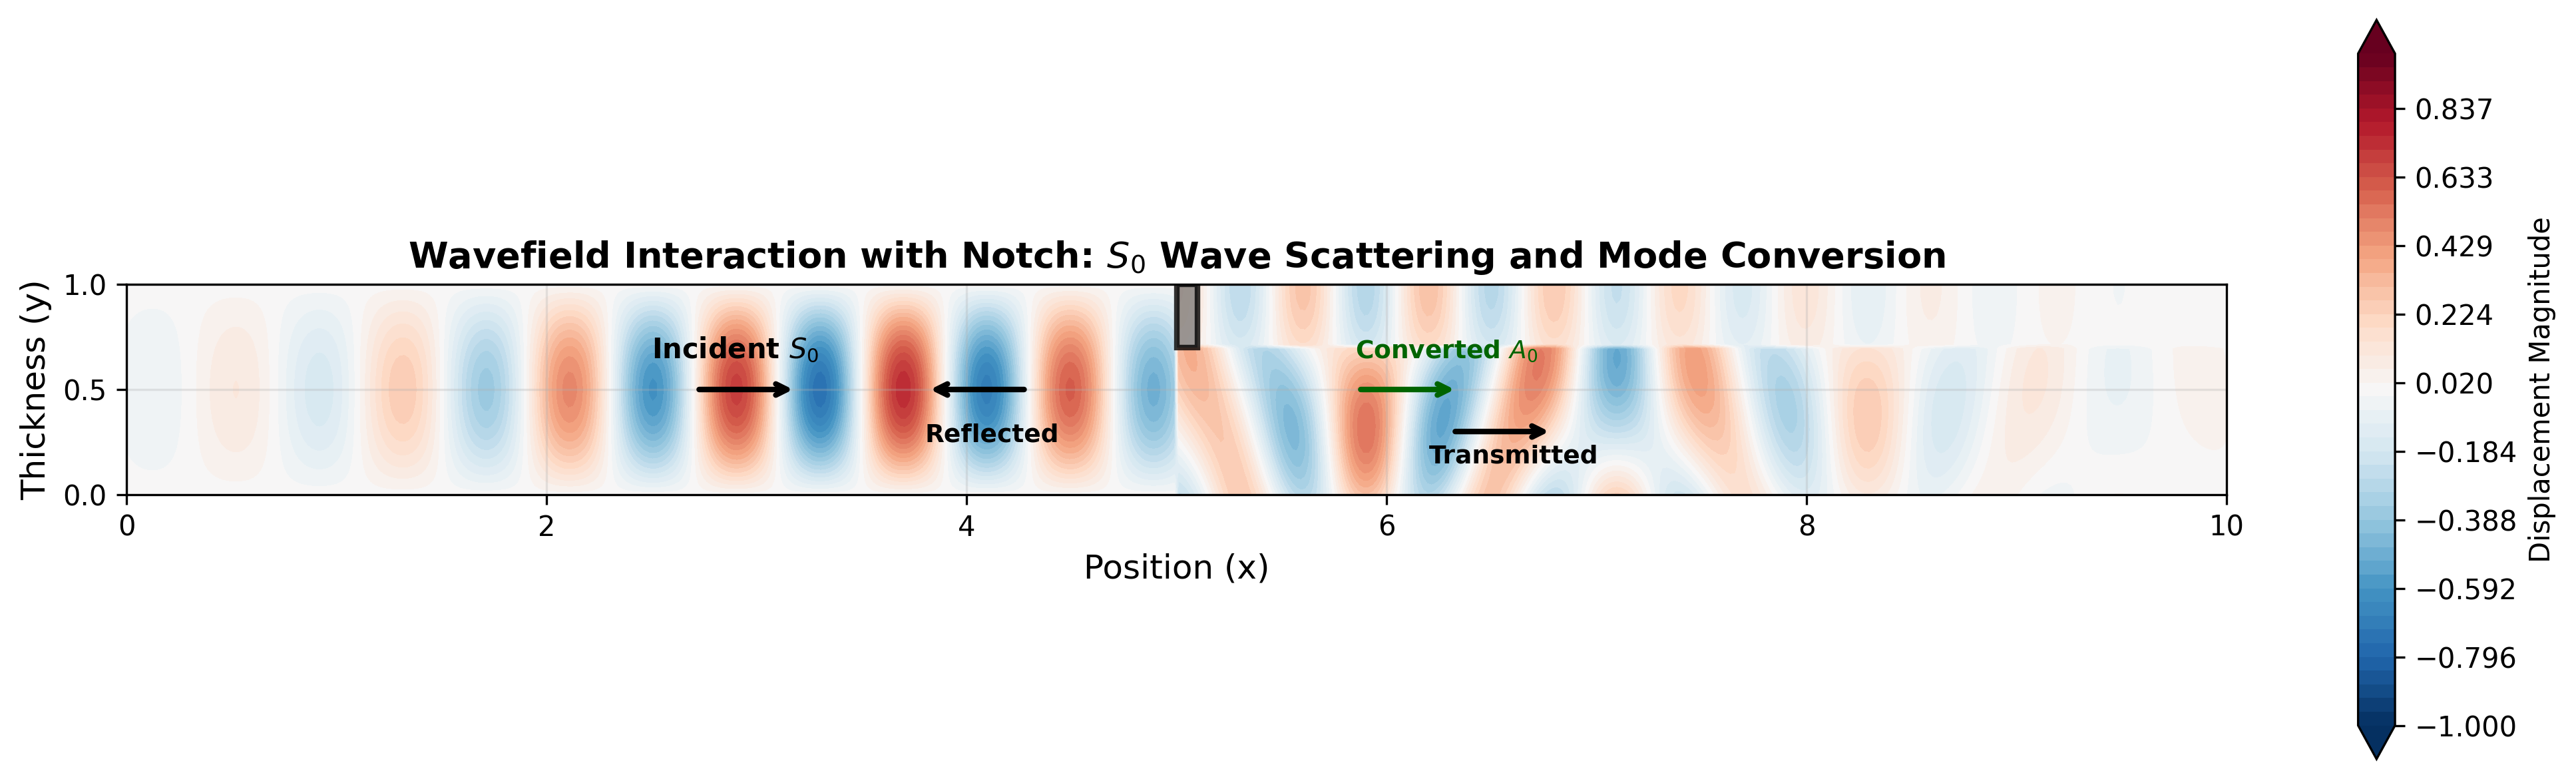
\includegraphics[width=1\textwidth]{Chapter2image/wavefield_notch.png}
\caption{Snapshot of wavefield interaction with a notch showing incident $S_0$ wave from left, reflected wave packet traveling backward, transmitted wave with reduced amplitude continuing forward, and mode-converted $A_0$ component propagating with different velocity. Color contours show displacement magnitude and arrows indicate wave fronts \citep{article}.}
\label{fig:wave_scattering}
\end{figure}

For notch-type defects, which are common in fatigue damage and manufacturing flaws, the scattering mechanism involves both the sharp geometric discontinuity at the notch edges and the reduced load-carrying capacity within the notch region. The notch creates a local flexibility, causing the structure to deform more readily under the incident wave's stress field. This enhanced deformation radiates secondary waves that comprise the scattered field. Deeper notches produce stronger scattering because they represent more significant impedance changes; wider notches scatter more energy because they interact with the wave over a larger spatial extent \citep{cawley2018practical}.

The temporal characteristics of scattered signals are equally important. When a transient pulse encounters damage, the reflected signal arrives back at the source location after a time delay determined by the damage location and the wave velocity \citep{rose2014ultrasonic}. If both $S_0$ and $A_0$ modes are present, each will have different arrival times due to their different group velocities, creating multiple reflection peaks in the time-domain signal. The temporal separation between these peaks provides redundant information about the defect location, improving robustness against velocity uncertainties \citep{na2021review}.

The complexity of scattering increases dramatically when multiple defects exist or when the damage has a complex three-dimensional geometry. Multiple scattering, where waves reflect between several defects, creates interference patterns that complicate interpretation. Delaminations or distributed damage produce diffuse scattering rather than specular reflection, requiring statistical or imaging-based analysis approaches \citep{cawley2018practical}. These complications motivate the development of inverse problem formulations where measured wave responses are used to infer damage parameters through optimization or machine learning, rather than attempting to analytically invert the scattering relationships.

\section{Use of Lamb Waves in Damage Detection}

Lamb wave-based damage detection involves generating waves through piezoelectric transducers, allowing propagation through the structure to interact with damage, and measuring the resulting wavefield at sensor locations~\cite{giurgiutiu2005}. Comparing measurements with baseline data or physics-based model predictions enables inference of damage presence, location, and characteristics.

Pulse-echo testing uses a transducer to generate a pulse that reflects from damage, returning after time delay $\Delta t$. The damage location $x_d$ relative to transducer position $x_0$ is:
\begin{equation}
x_d = x_0 + \frac{c_g \cdot \Delta t}{2}
\end{equation}
where $c_g$ is the group velocity and the factor of two accounts for round-trip travel. Multiple modes generate multiple reflection peaks, providing redundant distance measurements.

Pitch-catch configurations use separated actuator-sensor pairs~\cite{su2009}. Damage between transducers causes three signal changes: amplitude reduction in the direct path, additional scattered wave arrivals at intermediate times, and mode conversion introducing new modal components. The received signal is:
\begin{equation}
u_{\text{measured}}(x_s, t) = u_{\text{direct}}(x_s, t) + \sum_{i} u_{\text{scattered}}^{(i)}(x_s, t) + n(t)
\end{equation}
where $u_{\text{direct}}$ is the undamaged response, the sum represents scattering from all damage sites, and $n(t)$ is noise.

Triangulation using multiple transducer pairs enables localization~\cite{giurgiutiu2008}. Three or more pitch-catch measurements detecting the same defect create intersecting elliptical loci pinpointing damage location. Accuracy depends on transducer network density, time-of-flight precision, and velocity accuracy.

Damage characterization extracts quantitative defect information. Signal features correlating with damage include scattered wave amplitude (increasing with defect size), frequency content changes (larger defects scatter lower frequencies), and time-domain waveform shape (encoding defect geometry).

Damage indices quantify signal changes~\cite{su2009}. The correlation coefficient between baseline and damaged signals is:
\begin{equation}
\rho = \frac{\sum_{t} u_{\text{baseline}}(t) \cdot u_{\text{damaged}}(t)}{\sqrt{\sum_{t} u_{\text{baseline}}^2(t)} \cdot \sqrt{\sum_{t} u_{\text{damaged}}^2(t)}}
\end{equation}
Deviations from $\rho = 1$ indicate damage. Sophisticated indices combine multiple features to improve sensitivity and reduce false alarms from environmental variations.

The inverse problem approach seeks damage parameters $\boldsymbol{\theta}$ that reproduce measured signals when used in a forward model:
\begin{equation}
\boldsymbol{\theta}^* = \arg\min_{\boldsymbol{\theta}} \| u_{\text{measured}} - u_{\text{model}}(\boldsymbol{\theta}) \|^2
\end{equation}
This naturally handles complex damage geometries, multiple sensors, and multimodal propagation, but requires repeated forward model evaluations, motivating fast surrogate models to replace expensive finite element simulations.

Practical considerations affect detection success. Temperature variations shift arrival times, requiring compensation through ambient measurement or velocity-insensitive signal processing. Structural complexity creates additional reflections; baseline subtraction removes these but requires consistent measurement conditions. Spatial resolution is wavelength-limited: defects separated by less than approximately half a wavelength cannot be individually resolved, necessitating trade-offs between resolution (higher frequency) and range (lower frequency).

Integration of Lamb wave measurements with machine learning and surrogate modeling addresses traditional challenges. Data-driven models learn complex relationships directly from data, bypassing analytical scattering solutions. The multi-fidelity framework efficiently combines expensive high-fidelity simulations with abundant low-fidelity data, enabling rapid damage characterization for real-world monitoring. Following chapters develop these concepts, showing how computational and machine learning tools transform Lamb wave measurements into precise, quantitative damage assessments.

\section{Key Simulation Challenges}

While Lamb wave propagation physics is well-established, accurate numerical simulation of wave-damage interaction presents formidable computational challenges that motivate the surrogate modeling approach central to this thesis. These challenges stem from resolving wave phenomena across multiple spatial and temporal scales while maintaining numerical stability and accuracy.

The primary challenge is spatial discretization. Accurate wave propagation requires resolving the smallest relevant wavelength with sufficient mesh density. The standard rule demands at least ten to fifteen elements per wavelength to avoid numerical dispersion, artificial wave speed variations from discrete approximation. For high-frequency excitation or structures with small features like narrow notches, this forces extremely fine meshes. In a typical two-dimensional finite element model of a beam with length $L$ and thickness $h$, where thickness is orders of magnitude smaller than length, both directions need refinement. A 3-meter beam with 0.0015-meter thickness excited at 100 kHz might require elements smaller than 0.1-0.15 millimeters through the thickness to adequately resolve the Lamb mode shapes (requiring at least 10 elements through-thickness), while elements along the length could be somewhat larger but are typically kept on the same order to maintain reasonable aspect ratios. This results in tens of thousands of elements along the length and fine through-thickness discretization. The resulting system has millions of degrees of freedom even for this relatively simple geometry.

Temporal discretization compounds the burden. Explicit time integration schemes, commonly used for wave propagation due to their simplicity and efficiency, impose strict stability conditions on time step size. The Courant-Friedrichs-Lewy condition requires:
\begin{equation}
\Delta t \leq C \cdot \frac{\Delta x_{\min}}{c_{\max}}
\end{equation}
where $C$ is a stability constant typically around 0.5-0.8, $\Delta x_{\min}$ is minimum element size, and $c_{\max}$ is maximum wave speed. Fine spatial meshes force proportionally small time steps. Simulating wave propagation over structural dimensions—necessary to capture boundary and damage reflections—requires hundreds of thousands or millions of time steps. Each step involves matrix-vector operations whose cost scales with system size, making high-fidelity simulations expensive even with modern hardware.

Damage representation adds complexity. Sharp notches create geometric discontinuities requiring mesh refinement beyond wavelength criteria. Elements must conform to notch boundaries for accurate stress-free conditions, creating distorted elements near corners that degrade solution quality or further restrict stable time steps. Alternative approaches reducing material properties within the notch region rather than explicitly removing elements avoid remeshing but introduce calibration parameters. Moreover, parametric studies investigating various notch depths, widths, and locations require either multiple mesh generations or adaptive meshing strategies, both significantly increasing preprocessing burden.

Mode conversion during wave-damage interaction introduces fundamental modeling requirements affecting fidelity selection. Lower-order beam theories like Euler-Bernoulli or Timoshenko capture fundamental bending and extensional behavior but cannot represent through-thickness displacement and stress variation. Where mode conversion between symmetric and antisymmetric Lamb modes significantly affects scattered fields, these simplified theories may underpredict or misrepresent damage signatures. Higher-order theories or full two-dimensional continuum formulations capture mode conversion accurately but at substantially increased cost. This creates natural model fidelity stratification: fast one-dimensional models provide approximate responses for initial estimates or large parametric sweeps, while expensive two-dimensional models deliver reference solutions for validation and training data.

Numerical dispersion and dissipation, inherent discretization artifacts, corrupt solutions over long propagation distances or extended times. Even with adequate spatial resolution, cumulative numerical errors change wave packet shapes, with high-frequency components suffering disproportionate phase errors. Different finite element formulations—standard displacement-based elements, mixed formulations, spectral elements—offer varying balances between accuracy, cost, and implementation complexity.

The computational expense creates a critical bottleneck for inverse problems and uncertainty quantification. Solving an inverse problem to identify damage parameters from measured responses requires hundreds or thousands of forward simulations during optimization. Running each simulation for minutes or hours renders this impractical. Similarly, probabilistic assessments characterizing uncertainty in damage estimates require Monte Carlo sampling over parameter space, again demanding vast simulation numbers. This bottleneck motivates surrogate model development—fast, approximate representations of expensive simulations evaluable orders of magnitude faster while retaining sufficient accuracy for damage detection. Following chapters detail how combining different simulation fidelities with machine learning addresses these challenges, enabling practical solutions to forward and inverse problems in Lamb wave-based structural health monitoring.






\bibliographystyle{unsrtnat}
\bibliography{ref} 
\end{document}